% brokers_who_do_not_bridge_without_appendices.tex: GENERATED, do not edit.
% Built by scripts/paper/build_manuscript.jl on 2026-09-01T05:40:42.695.
% Manuscript commit: c4a355d3fa41aee2772e8217e1bd89d99bad1059; uncommitted manuscript/build changes included.
% The editable root is paper/brokers_who_do_not_bridge_without_appendices.tex; the results provenance is
% recorded in the inlined output/main/results_section.tex header below.

% Converted from the original Word draft with Pandoc 3.10.1.
% Word tracked changes were accepted, and embedded Zotero citation fields were
% linked to paper/references.bib, a mechanically extracted subset of the
% verified PHD.bib reference-library export.
% Editable root for the complete manuscript. The results section is generated
% separately and included below. Use scripts/paper/build_manuscript.jl to create
% the flattened, submission-ready TeX bundle under output/manuscript/.

% Options for packages loaded elsewhere
\PassOptionsToPackage{unicode}{hyperref}
\PassOptionsToPackage{hyphens}{url}
\documentclass[
]{article}
\usepackage[letterpaper,margin=1.25in]{geometry}
\usepackage{xcolor}
\usepackage{amsmath,amssymb}
\usepackage{graphicx,booktabs}
\usepackage[font=small,labelfont=bf]{caption}
\usepackage{fancyhdr}
\graphicspath{{./}}
\setcounter{secnumdepth}{5}
\usepackage{iftex}
\ifPDFTeX
  \usepackage[T1]{fontenc}
  \usepackage[utf8]{inputenc}
  \usepackage{textcomp} % provide euro and other symbols
\else % if luatex or xetex
  \usepackage{unicode-math} % this also loads fontspec
  \defaultfontfeatures{Scale=MatchLowercase}
  \defaultfontfeatures[\rmfamily]{Ligatures=TeX,Scale=1}
\fi
\usepackage{lmodern}
\ifPDFTeX\else
  % xetex/luatex font selection
\fi
% Use upquote if available, for straight quotes in verbatim environments
\IfFileExists{upquote.sty}{\usepackage{upquote}}{}
\IfFileExists{microtype.sty}{% use microtype if available
  \usepackage[]{microtype}
  \UseMicrotypeSet[protrusion]{basicmath} % disable protrusion for tt fonts
}{}
\makeatletter
\@ifundefined{KOMAClassName}{% if non-KOMA class
  \IfFileExists{parskip.sty}{%
    \usepackage{parskip}
  }{% else
    \setlength{\parindent}{0pt}
    \setlength{\parskip}{6pt plus 2pt minus 1pt}}
}{% if KOMA class
  \KOMAoptions{parskip=half}}
\makeatother
\setlength{\emergencystretch}{3em} % prevent overfull lines
\providecommand{\tightlist}{%
  \setlength{\itemsep}{0pt}\setlength{\parskip}{0pt}}
\usepackage[style=authoryear-comp]{biblatex}
\addbibresource{references.bib}
\renewcommand{\thesection}{\Roman{section}}
\renewcommand{\thesubsection}{\Alph{subsection}}
\usepackage{bookmark}
\IfFileExists{xurl.sty}{\usepackage{xurl}}{} % add URL line breaks if available
\urlstyle{same}
% fallback for those not using the hyperref driver hyperxmp:
\makeatletter
\@ifundefined{xmpquote}{\newcommand{\xmpquote}[1]{#1}}{}
\makeatother
\hypersetup{
  pdftitle={Brokers Who Do Not Bridge: When Assessment{,} Not Access{,} Shapes Broker Advantage},
  pdfauthor={Marie-Lou Laprise},
  hidelinks,
  pdfcreator={LaTeX via pandoc}}

\newcommand{\latestcompleteversionurl}{https://raw.githubusercontent.com/m-laprise/brokerage-abm/main/output/manuscript/brokers_who_do_not_bridge_with_appendices.pdf}
\fancypagestyle{workingpaperfirst}{%
  \fancyhf{}
  \renewcommand{\headrulewidth}{0pt}
  \renewcommand{\footrulewidth}{0pt}
  \fancyfoot[C]{\footnotesize This version: \today. Get the latest version: \href{\latestcompleteversionurl}{\textcolor{blue}{link}}.}
  \fancyfoot[R]{\footnotesize\thepage}
}

\title{Brokers Who Do Not Bridge: When Assessment, Not Access, Shapes Broker Advantage}
\author{Marie-Lou Laprise}
\date{}

\begin{document}
\maketitle
\thispagestyle{workingpaperfirst}
\begin{abstract}
Structural theories describe economic brokerage as an opportune but fragile position bridging gaps between otherwise disconnected actors. In that view, brokering can undermine trust or eliminate the gaps that generate its value, and brokers need supporting institutions or deeper interpersonal ties to stabilize their role. Yet many corporate actors in positions of brokerage, from Visa to Amazon, have risen in market power, profit, and prominence even as networks transformed around them. When can brokering strengthen rather than undermine a broker's advantage?

I reconceptualize brokerage as outsourced relational work, in which a broker who assumes no inventory risk constructs viable matches between parties who cannot easily find or evaluate one another. Repeated matchmaking generates an informational byproduct that the broker can accumulate: knowledge of what makes pairings successful across the market, unavailable to clients who observe only their own dealings. An agent-based model of a matching market identifies conditions under which this informational advantage emerges and persists. Brokerage can provide assessment rather than access: clients outsource matching even when they can reach counterparties themselves, because the broker's predictions are valuable. Counterintuitively, the broker can become highly central in regimes where it engages in little bridging behavior: broker centrality is a product, not a primary source, of matchmaking quality.

While the model explores the dynamics of the broker's informational advantage, I theorize how this advantage can then enable the broker to become a principal selling the resource it once intermediated or monetizing data and analytics. This is \emph{transient brokerage}, a process that highlights a broker's growing power rather than its fragility.
\end{abstract}

\section{Introduction}

Intermediation in economic relations---the intervention of a third party to mediate or facilitate exchange between others---can take many forms, including that of brokerage. Brokers are intermediaries that do not assume inventory risk: they act as matchmakers, connecting others.

Brokerage is pervasive in a wide variety of markets and remarkably persistent across time and space. Brokers find themselves in an advantageous but delicate position. Unlike dealers and wholesalers, brokers do not sit on an inventory that they need to manage and can liquidate in case of difficulty. Unlike market makers, they keep offers and price information private \autocite{rustMiddlemenMarketMakers2003}. They operate at the intersection of social groups \autocite{burtStructuralHolesSocial1992,burtStructuralHolesGood2004} and rely on secret information. As a result, they often lose the trust and legitimacy needed to continue their activities. Prominent theories of brokerage have described it as an opportune but inherently fragile role that often gets ``stabilized'' to avoid collapsing, through the social isolation of brokers, their organizational grafting, or their capture by one side \autocite{stovelStabilizingBrokerage2011}.

If that is the case, then how have so many corporate actors in positions of brokerage, from Visa to Amazon, managed to rise in market power, profit, and prominence even as networks transformed around them and could have undercut them?

Recent work by Ronald S. Burt, building on the tradition of structural-hole brokerage theory, has shown one important reason why the broker fragility narrative fails: many bridging ties are not weak and fragile, but rather strong high-trust ties forged through interpersonal history, and they provide a robust and enduring advantage to the broker who relies on them \autocite{burtFragileBrokerage,burtStrongBridgesTrust2026a}. However, this is not the full story.

Some brokers leverage their role to become principals rather than remain only intermediaries. In so doing, they stabilize their advantage and consolidate power while brokering becomes secondary or even disappears entirely. I call this \emph{transient brokerage}, a phenomenon which current theories of brokerage do not satisfactorily predict or explain. Transient brokerage highlights how brokering sometimes declines or disappears because of the broker's power, not its fragility.

To explain transient brokerage, this article redefines brokerage as \emph{outsourced relational work}: the broker constructs viable matches between parties who cannot easily find or evaluate each other. This relational work generates an informational byproduct that the broker can leverage. Structural position provides the access that feeds learning, but while each successful match between previously unconnected parties can erode the broker's structural advantage by densifying the network \autocite[356]{burtNetworkStructureSocial2000}, it also strengthens the broker's informational position. The broker accumulates knowledge of what makes pairings successful.

In that way, the broker converts structural capital into informational capital through the act of brokering. This is particularly true for corporate brokers, who operate at scale and whose relational work benefits from legal privileges conferred by the corporate form. Depending on the market in which the broker operates, the nature of the matching problem, and the relations between the actors involved, the broker's information advantage can support a transition from intermediation to capture. The broker dismantles the relational package that was negotiated with its principals and converts vicarious relational work into personal economic advantage. If successful, \textbf{the broker becomes a principal} \textbf{selling} \textbf{the resource it once intermediated} \textbf{or} \textbf{monetizing data and analytics}. \emph{Corporate} relational work is a particularly advantageous basis for such capture. This explains the rise in prominence of some firms acting as brokers

This article shows how the broker builds and sustains an informational advantage, through social theory illustrated by computational simulations, and explains how this advantage can then enable the broker to transition from intermediary to principal. It attempts to answer three questions about brokerage, generating propositions to be tested in future empirical work:

\begin{enumerate}
\def\labelenumi{(\roman{enumi})}
\item
  What value does a broker provide?
\item
  How does brokering alter its informational and structural position?
\item
  Under what conditions can the broker convert its advantage into resource capture or data enclosure?
\end{enumerate}

I develop an agent-based model (ABM) of brokerage in a general matching market and use it to formalize and illustrate how brokers create and preserve an informational advantage through repeated matchmaking. The simulations show how several simple elements interact to produce non-obvious dynamics, and they complicate the expectation that brokers densify networks around them and erode their own position. The results suggest that brokerage can provide assessment rather than access and that clients continue outsourcing even when they can reach counterparties themselves. A broker's structural prominence can be produced endogenously by its success in the work it performs, centrality is separate from actual bridging behavior, and a broker need not liquidate its own structural position. A broker can be highly central while engaging in little to no bridging. The results recast betweenness centrality not as a neutral measure of a broker's strength grounded in network topology, but as a product of the kind and quality of its relational work.

The rest of this article proceeds as follows. Section II reviews structural and processual theories of brokerage and their blind spots. Section III reconceptualizes brokerage as outsourced relational work and traces how this work is transformed when performed at scale by corporate actors. Section IV presents the ABM and its results illustrating how a broker produces and sustains their advantage through this work. Section V builds on this foundation to theorize one possible trajectory that can follow from the broker advantage, transient brokerage, and the conditions under which a broker can become a principal. Section VI discusses scope conditions and implications for the political economy of corporate intermediation, and Section VII concludes.

\section{Current Theories of Brokerage Do Not Explain Capture by the Broker}
\label{sec:brokerage-theory}

Brokerage tends to emerge in markets where information is scarce or complex, participants are few, transactions are intricate, or institutions are poorly developed \autocite{stovelStabilizingBrokerage2011}. These conditions make participants hard to find, resources hard to value, or transactions hard to structure. They also make the intermediation work of a broker valuable. Real estate, mortgage, stock, and commodity markets are common examples of markets with many active brokers. Brokerage may also be helpful in circumstances where tight-knit, closed groups monopolize resources or information, and outsiders cannot easily access them \autocite[140]{stovelBrokerage2012}. Brokerage can maintain or reinforce group boundaries, or it can blur or collapse them \autocite{stovelBrokerage2012}, with consequences for social segregation, social integration, and relations between groups or communities \autocite{galsterWordsDeedsRacial2005}.

Past research has proposed two conflicting sets of definitions of brokerage \autocite[see][for a review]{eriksonFormalistRelationalistTheory2013}: narrower formalist or structuralist definitions \autocite{burtStructuralHolesSocial1992,gouldStructuresMediationFormal1989,granovetterStrengthWeakTies1973,marsdenBrokerageBehaviorRestricted1982}, and broader processual definitions \autocite{obstfeldBrokerageProcessDecoupling2014,rossmanObfuscatoryRelationalWork2014,spiroExtendedStructuresMediation2013,stovelBrokerage2012}.

\subsection{Formalist and Structuralist Definitions}

Early brokerage research examined the structure of networks and the positions of actors to identify brokerage forms, categorize them, and determine their consequences \autocite{burtStructuralHolesSocial1992,burtStructuralHolesGood2004,gouldStructuresMediationFormal1989,granovetterStrengthWeakTies1973,marsdenBrokerageBehaviorRestricted1982,simmelConflictWebGroupAffiliations1964,simmelIndividualitySocialForms1971}. Brokerage opportunities arise when there are gaps in a social network, such that some nodes are close (in degrees of separation) yet disconnected \autocite{burtStructuralHolesSocial1992,burtStructuralHolesGood2004,marsdenBrokerageBehaviorRestricted1982}. Brokerage is synonymous with open triads or structural holes: a structure in which a third actor bridges two otherwise unconnected nodes. The third actor mediates flows of resources and information and facilitates transactions between others who lack access to one another \autocites[1457]{fernandezDilemmaStatePower1994}[202]{marsdenBrokerageBehaviorRestricted1982}. Researchers in this tradition generally set aside interactional content to achieve greater generality \autocite{eriksonFormalistRelationalistTheory2013}. For instance, \textcite[36]{burtStructuralHolesSocial1992} was explicit in treating ``motivation and opportunity as one and the same.''

\textcite{burtStructuralHolesSocial1992} operationalized the structural-hole concept, proposing the measures of network constraint and effective size to quantify how well positioned an actor is for brokerage, which allowed the theory to be tested across a wide range of settings. For instance, in a follow-up study, \textcite{burtStructuralHolesGood2004} investigated the network position of 673 managers in a large electronics company. He found that those who spanned structural holes generated ideas that senior management judged more valuable and were rewarded with better performance evaluations, promotions, and compensation. He suggested that brokers appear more creative because they can take insights that are commonplace in one group and introduce them to other people to whom they appear novel and original \autocite[388]{burtStructuralHolesGood2004}.

As such, brokers derive an advantage from their ability to exploit pre-existing information in the network. Because of their position, brokers get privileged access to diverse ideas from across the network. They can see opportunities that others do not, and they can strategically use their position by providing or withholding information \autocite{burtStructuralHolesSocial1992} or using it to sustain their own creative endeavors. Exposed to varied perspectives, they are well-positioned to build a richer understanding, synthesize across domains or outlooks, and develop a unique vision \autocite{burtStructuralHolesGood2004}.

Defining brokerage based on structural holes, however, excludes situations that clearly appear as brokerage to a lay observer. For instance, Alice wants to sell her house and asks a real estate broker to list it. Soon after the real estate broker puts up the `for sale' sign, her neighbor Bob, whom she knows personally, contacts the broker to purchase the house. A broker intermediates the transaction, yet no structural hole existed between buyer and seller.

\subsection{Processual Definitions}

More recently, some researchers have recast brokering as a set of relational processes \autocite{obstfeldBrokerageProcessDecoupling2014,rossmanObfuscatoryRelationalWork2014,spiroExtendedStructuresMediation2013,stovelBrokerage2012}. Stovel and Shaw suggested that brokerage was ``the process of connecting actors in systems of social, economic, or political relations in order to facilitate access to valued resources'' \autocite[141]{stovelBrokerage2012} \autocite[see also][]{stovelStabilizingBrokerage2011}. Brokers exhibit two crucial features: they are positioned as bridges across gaps, and they help transfer resources or knowledge across those gaps \autocite[141]{stovelBrokerage2012}. This definition remains constrained by social structure but requires brokerage behavior. Hence, there can be structural holes without brokerage---some bridging actors do not transmit anything across holes---but no brokerage without structural holes. In this way, it runs into the same conceptual problem as purely structural definitions.

\textcite{obstfeldBrokerageProcessDecoupling2014}, building on Marsden \autocite*{marsdenBrokerageBehaviorRestricted1982}, proposed a purely processual definition: brokerage is a process by which an actor ``alters interaction between two or more parties in a wide variety of triadic structures'' \autocite[136]{obstfeldBrokerageProcessDecoupling2014}, meaning that he ``influences, manages, or facilitates'' the interaction \autocite[141]{obstfeldBrokerageProcessDecoupling2014}. This eliminates any structural requirement beyond the need for three or more actors. It is no longer necessary for the alters to lack access to or trust in each other. There can be structural holes without brokerage, and there can also be brokerage without structural holes: brokerage behavior can, and often does, occur in dense networks.

Previous work on brokerage, particularly in the processual tradition, has also identified categories of brokers depending on the nature of their activities. Middleman, transfer, or conduit brokers facilitate economic transactions without necessarily altering the structure of a local network, like stockbrokers \autocite[146]{stovelBrokerage2012} \autocite{spiroExtendedStructuresMediation2013} \autocite[141]{obstfeldBrokerageProcessDecoupling2014}. Catalyst, moderator, or matchmaking brokers focus on creating lasting ties, like headhunters and party hosts \autocite[146]{stovelBrokerage2012} \autocite{obstfeldBrokerageProcessDecoupling2014} \autocite{spiroExtendedStructuresMediation2013}. Finally, \emph{coordinators}, such as middle managers or disaster response teams, work to transform existing ties by reconfiguring local networks of interdependence \autocite[131-132]{spiroExtendedStructuresMediation2013}.

While definitions based on structural holes were very restrictive, Obstfeld and co-authors' processual definition is sweeping. For instance, they suggested that, under their definition, a manufacturing firm acts as a broker when it buys raw materials from an alter, transforms them into a product, and sells the finished product to another alter \autocite[145]{obstfeldBrokerageProcessDecoupling2014}. Most triadic or polyadic relations, in this account, imply brokerage. Indeed, many descriptions of brokers in the literature are so broad as to invite the charge that a concept that explains everything explains nothing. The most varied social facts have been described as acts of brokerage: mediating conflict \autocite{obstfeldBrokerageProcessDecoupling2014}, reselling stolen property \autocite{steffensmeierFenceShadowTwo1986}, advocating on behalf of someone, making sense of the world for someone, and helping connect epistemic communities \autocite[140]{stovelBrokerage2012}, to name only a few.

\subsection{Shortcomings of Existing Frameworks}

Work that relies chiefly on the structural holes idea generally makes clear that transferring knowledge and ideas is a key element of brokering and of the broker advantage. Yet, the information being considered is generally pre-existing, ambient information, not the one that the process of brokering generates \autocite{burtStructuralHolesGood2004}. Moreover, the structural account leaves the actual work of brokering largely implicit. Structural position indicates places where brokerage is possible, but not whether anyone is doing the work of brokering---work for which structural holes are neither necessary nor sufficient.

Meanwhile, broad processual definitions blur the lines between vicarious and personal relational work. They include under the same umbrella cases where the intermediary deals with others on its own account, and cases where the intermediary works on behalf of others. As such, this perspective doesn't examine the informational byproduct that results from repeated vicarious work. Information is often simply listed among the resources that can be transferred through a broker, along with material or financial resources \autocites[see e.g.][141]{obstfeldBrokerageProcessDecoupling2014}[141]{stovelBrokerage2012}.

Neither perspective offers a cohesive theory of the role of information in brokerage, even though information shapes every stage of the brokering process. Before brokerage, the distribution of information shapes the opportunity or need for it: brokerage arises partly out of informational inequality, and the broker exploits what it knows that one or both sides do not. During brokerage, the transmission of information is part of the brokerage act itself, as the broker shares enough to make a match viable while withholding enough to preserve its advantage. After brokerage, the distribution of information has been altered, and the work has generated a byproduct the broker retains, which may shape the broker's opportunities. The circulation of information is at once a determinant of brokerage, a component of the work of brokering, and a consequence of brokerage.

This article reconceptualizes brokering as outsourced relational work and builds on this theoretical move to explain how brokerage sometimes weakens or disappears because a powerful broker captures resources or encloses data to become a principal.

\section{Outsourced Relational Work and the Broker Advantage}

Social actors engage in \emph{relational work} when they try to interpret and match social ties, economic transactions, and media of exchange, to create viable matches that will shape the outcome of their interaction \autocites[151]{zelizerHowBecameRelational2012}{zelizerPurchaseIntimacy2005} \autocite[see also][255]{bandeljRelationalWorkEconomy2020}. These matches and their shared meanings form distinct \emph{relational packages}. For instance, in a marketplace, actors trading directly with one another draw on cultural knowledge to reach a shared understanding of their situation and the `rules of the game,' and to agree on terms, including price \autocite[137]{blockRelationalWorkMarket2012}.

For the broker's clients, brokerage is \emph{outsourced} \emph{relational work}. For the broker, brokerage is \emph{vicarious relational work}. In economic markets, this outsourced relational work is usually performed at scale by a \emph{corporation}. This is more than a question of definitions: it shapes the broker's opportunities, its strategic advantage vis-à-vis its clients, and its trajectory.

\subsection{\texorpdfstring{From Personal to \emph{Outsourced and Vicarious} Relational Work}{From Personal to Outsourced and Vicarious Relational Work}}

In brokered transactions, brokers take on the work of constructing a shared reality for limited purposes. The core of what brokers do is relational matching \autocite[see][]{zelizerHowBecameRelational2012}. Brokers are characterized by the relational work they do \emph{on behalf of others}.

For the broker, this vicarious work requires another layer of relational work to negotiate brokerage relations with its clients. Brokerage corresponds with a distinct relational package. Not all intermediation is brokerage. In the relational package of economic brokerage, the broker performs a matching service for others, usually for a fee, commission, or retainer. Brokers bundle various services and amenities as part of that package: they take on the efforts of search and negotiation, they provide access to otherwise inaccessible counterparties, they share with their clients their expertise and the benefits of the private information they hold about quality, pricing, and availability, and they document and facilitate transactions, which often require logistical, bureaucratic, or regulatory work.

The middleman, catalyst, and coordination brokerage described in Section~\ref{sec:brokerage-theory} are not exclusive categories of brokers, but rather, components of the work of brokering, which involves a bit of each in varying proportions. An important part of brokers' relational matching is to facilitate interaction (middleman brokerage), but this work also directly impacts interpersonal relations and local networks, often in an enduring way, by creating new and lasting ties (catalyst brokerage) or by reorganizing local networks (coordination brokerage).

Brokerage inherits the dual character of relational work, which can both foster and reduce informational asymmetry when constructing shared understandings while maintaining strategic opacities \autocite[138]{blockRelationalWorkMarket2012}. In performing relational work on behalf of others, the broker simultaneously clarifies and obscures: it transmits enough information to make a transaction legible and a match viable and conceals enough to justify its fee and preserve its advantage. The same opacity can do social as well as economic work. Rossman \autocite*{rossmanObfuscatoryRelationalWork2014} shows how brokerage functions as obfuscatory relational work that manages the taboos around disreputable exchange. Outsourcing relational work provides cover to parties in morally fraught matches. What the broker withholds is also the raw material of its later advantage: information it keeps from circulating, accumulates, and, under the right conditions, eventually monetizes.

Vicarious work relates to entities or resources that are \emph{not} under the broker's personal ownership and control, and the shared understanding of the parties is that the broker is \emph{not} \emph{a principal} in the brokered transaction \autocite[see e.g.][21326]{stovelStabilizingBrokerage2011}. Brokers generally have limited personal involvement in brokered interactions beyond their role as facilitators. The broker is a supporting actor, not a main character. Intermediaries who have full control over traded resources occupy a very different position in terms of risk, power, and vulnerability.

Another way to put it is that in economic markets, brokers are intermediaries that \emph{do not assume inventory risk}. That is, if Bob helps Alice and Charlie conclude a sale, Bob is a broker. If Bob buys from Alice and eventually leases to Charlie, he is not. For instance, a real estate broker using her market knowledge to buy houses in up-and-coming neighborhoods to rent to families no longer acts as a broker. Instead, the relational work she performs is personal: matching herself to sellers and renters.

\subsection{\texorpdfstring{From Individual to \emph{Corporate} Relational Work}{From Individual to Corporate Relational Work}}

The definition above applies naturally to describe individual brokers working with individual clients, such as a real estate agent, an insurance broker representative, or a matchmaker. Much of the work of brokerage, however, occurs at the corporate, organizational, or institutional level, where brokers are firms, and clients may also be.

To understand what happens when relational work is outsourced to corporations, we must first discuss how corporations perform relational work in the first place, for themselves as organizational social actors. Relational work scholarship initially focused on the intimate sphere and interpersonal relationships \autocite[see][for a review]{bandeljRelationalWorkEconomy2020}. But relational work also takes place in the economic sphere and at the organizational level. The relational work tradition has acknowledged the organizational question without fully resolving it. Bandelj \autocite*{bandeljRelationalWorkEconomic2012} noted that relational work between representatives of organizations solidifies into macrolevel structures, while Zelizer \autocite*[156-157]{zelizerHowBecameRelational2012} catalogued instances of relational work by firms in the field of labor relations. Bandelj's \autocite*{bandeljRelationalWorkEconomy2020} review of ``scaling up'' relational work surveyed studies operating at the organizational level, but they mainly focused on what people do with and to each other within organizations, not on the corporate form itself as a vehicle for relational work.

Firms must conduct relational work to manage contingent, fleeting ties and longer-term relationships with workers, consumers, suppliers, lenders, investors, bureaucrats, and so on. The properties of the corporate form matter to this work and make it distinct. The firm is not simply a site where interpersonal relational work occurs; nor is it a singular, scaled-up actor that performs relational work like an individual would.

Firms are groups of people in designated roles, following norms and practices, supported by procedures, interfaces, and infrastructures, and doing the everyday work of managing the firm's relationship with its environment ``at the coalface'' \autocite{grayGoverningOrganizationInterpreting2014,huisingNudgeCultureBack2018}. The mining metaphor directs attention to the frontline of the organization, where people enact its dealings with the outside world and translate organizational imperatives into routine practice. Relational work, like everything the corporation does in the world, is enacted through the people, procedures, infrastructure, and algorithms working at the coalface. Because of its collective and distributed nature, it is never visible in its entirety to any of the people involved.

Most firms are also legally organized as corporations. The corporation is a political entity with emergent capacities for coordination, information processing, and strategic action that exceed the sum of its parts \autocite{ciepleyPublicPrivatePolitical2013a,farrellUndergroundEmpireHow2023}. There is a fundamental asymmetry between corporate actors and natural persons \autocite{colemanAsymmetricSociety1982,colemanFoundationsSocialTheory1990}. The corporation aggregates information across thousands or millions of interactions, while each natural person sees only their own. The corporation can persist indefinitely, while individual relationships are transient. The corporation coordinates strategically across its full portfolio of relationships, while each counterparty acts in isolation. As a result, when a corporate actor interacts with natural persons, the corporate actor has structural and informational advantages.

These asymmetries are not accidental byproducts of size: they are legally constituted features of the corporate form. The corporation is one of the core modules of the legal code of capital \autocite{pistorCodeCapitalHow2019}. Corporate law endows the firm with durability that outlasts any individual relationship, priority that ranks its claims above those of other parties, and universality that makes those claims enforceable against the world, so that it can become a legal technology for concentrating and protecting accumulated advantages and leveraging them for productive purposes. These are the conditions under which corporate relational work takes place: it is inherently asymmetric, because of the different scales and material and informational resources of corporate and natural persons.

\subsection{Outsourcing Relational Work to Corporations: The Corporate Brokers}

When a client outsources relational work to a corporate broker, the corporate broker performs that work through people and practices at the coalface, each working in some small way to define relational packages, perform appropriate matches, and shape information flows. The corporate form reorganizes vicarious relational work, distributes it across roles, and embeds it in routines and procedures. To orchestrate this, corporate brokers develop an organizational apparatus comprised of internal and client-facing roles, information architectures and databases, contractual templates, and interfaces.

Saying a brokerage firm does relational work on behalf of its clients means that in sales meetings, in contract negotiations, in the design of user interfaces, in the defaults embedded in terms of service, and so on, people relying on organizational procedures are working to define the features of its clients' relationships, what transactions are appropriate to them, and what media may govern the exchanges. Just like for its own relational work, the corporation has a capacity for coordination, information aggregation, and temporal persistence that makes the vicarious relational work of corporate brokerage qualitatively different from what any individual could accomplish alone.

The corporate broker's relation with its clients is structurally asymmetric. With human clients, corporate and natural persons bring fundamentally different legal, informational, and temporal architectures to the relationship. Even with corporate clients, however, the asymmetry remains: the broker coordinates vicarious relational work strategically and benefits from cross-market information, while the client encounters it piecemeal. The matching of relations, transactions, and media moves from a pure negotiation between principals with comparable standing, who learn from each transaction, toward an administered process in which the corporate broker sets the terms, explicitly or behind the scenes, and captures the information that each pairing generates.

The data infrastructure of the corporate broker includes data taxonomies, client categories, risk models, algorithmic sorting procedures, and so on. This infrastructure does not merely facilitate transactions but actively constitutes relational packages by determining what transactions are possible, and what categories they should fall into. Classification systems and information infrastructures, like that of the corporate broker, are not neutral descriptions of the world; they actively organize social relations \autocite{fourcadeOrdinalSociety2024,geoffreyc.bowkerSortingThingsOut1999}. The corporate broker's information infrastructure, much like a corporate rating agency's credit-scoring system or a platform's matching algorithm, sorts counterparties into categories the broker defines and uses those categories to allocate opportunities according to the broker's objectives. The impact of the broker's information infrastructure is magnified because the corporate broker works at scale, while individuals cannot usually design categories that simultaneously structure millions of relationships.

\subsection{The Broker Advantage}

Why do people and firms outsource their relational work to brokers? To have the opportunity to broker, a participant in a matching market must hold either a \emph{structural} or an \emph{informational} advantage. The structural advantage depends purely on network topology and should translate into \emph{access}: the broker can reach counterparties that clients cannot. The informational advantage should translate into \emph{assessment}: the broker can evaluate prospective matches better than its clients can. In other words, the broker's service is valuable because it helps the client match with counterparties that the client could not otherwise easily find \emph{or} evaluate.

Assessment involves two components: evaluating the general quality of the goods or counterparties involved and evaluating the quality of the specific pairing or relational package being considered. These components also correspond to two possible channels for the broker's information advantage: \emph{attributional}, about how parties' attributes translate into individual quality, and \emph{relational}, about which counterparties complement each other. Both are self-reinforcing, as the broker accumulates the knowledge required for assessment through the relational work it performs, and that learning makes it better at the work. The broker observes outcomes from many pairings across many principals, while each principal observes only its own. This gives the broker both a cross-market view and higher data volume.

The broker's information work can be informal and internal, as with a real estate broker who knows the local market, has an intuition for the right asking price, and holds social ties to likely buyers. It can also be formal and bureaucratized, as with a corporate mortgage broker that follows tables and formulas to determine which interest rate may produce successful matches between borrowers and lenders. The latter records and retains what the former holds only in personal experience, and this difference reflects that between individual and corporate brokerage.

Important models in the economics literature have focused on the attributional channel and characterized the broker's role primarily as quality certification \autocite{liMiddlemenPrivateInformation1998} or expert screening \autocite{bethuneInformationbasedTheoryFinancial2022a}: the broker identifies which goods or counterparties are high quality. In that view, the broker is an appraiser whose cross-market experience helps it assess the general quality of counterparties more accurately than individual principals can. The relational-work view of brokerage suggests that the broker's value lies also, and often primarily, in understanding complementarities between counterparties and shaping relational packages accordingly. The broker is a relational worker and a matchmaker whose advantage comes from the ability to make pairings and to know which pairings will likely succeed, an ability that improves with repeated matchmaking.

% Generated from paper/section_source.tex by scripts/paper/build_section.jl.
% results_section.tex: GENERATED, do not edit.
% Built by scripts/paper/build_section.jl on 2026-09-01 05:40
% from section_source.tex + captions.tex + values.tex + convergence/values.tex +
% Ridge and ablation values + figmeta.tex;
% sweep 2026-08-30_e5b9858_combined_20_baseline50; analysis commit c75e9d1e5487884bf82e80a3a232f4c769c66404;
% manuscript commit c4a355d3fa41aee2772e8217e1bd89d99bad1059; uncommitted manuscript/build changes included.
% Every number was computed from the saved sweep data by the reporting scripts.

\section{ABM Results: The Broker's Advantage in a Simulated Matching Market}

\subsection{Model and Methods}

To formalize and illustrate the theory developed in this article, this
section describes an ABM of brokerage in a general matching market and
presents the results of exploratory computational simulations. Their
purpose is not to prove or disprove the theory, but to operationalize
it, explore the dynamics it entails while providing concrete
illustrations to the reader, and generate falsifiable propositions that
future empirical work can use as hypotheses.

The theory makes claims about trajectories and feedback among
heterogeneous, boundedly informed actors interacting repeatedly, making
the ABM a natural tool to make its mechanisms explicit and sharpen its
propositions.

The model is domain-agnostic and represents any market in which a broker
facilitates pairwise matches and accumulates cross-market data from
doing so. All agents use heuristic decision rules, and no agent is
perfectly rational. One period equals one full update of the simulation
loop; each period could be taken to represent one calendar month, one
week, or one day, for instance, depending on the pace of the market that
one wants to represent.

Pseudo-code and complete specifications for the model are included as
\textbf{Appendix A and B}, respectively, and the code base for the project,
implemented in Julia, is publicly available at
\texttt{https://github.com/m-laprise/brokerage-abm}. It includes the
scripts needed to reproduce the experiments that generated the data
analyzed in this section, extract every number mentioned, create the
figures and tables, and generate the results section in its entirety.

\emph{Setup}. Many principals and a single broker, connected through an
undirected network, inhabit the market. Each period, a principal draws a
demand for new pairwise matches. Principals seeking matches search on
their own for counterparties (self-search channel) or outsource to the
broker (broker channel). The decision is made by comparing a running
satisfaction score for each channel; principals who have never used the
broker rely on its reputation (average satisfaction of current clients).
After each period, each agent exits with probability $\eta$ and is
replaced by a fresh entrant.

\emph{Nature of the matching problem} (Appendix B \S2). Each principal has a
fixed type, a vector of observable characteristics. A realized match
between two principals yields an output equal to a fixed function of the
two parties' types plus noise. The signal is unknown to everyone and
must be learned. It has two parts, combined by a mixing weight $\rho$. The
first is a general-quality term computed as the average of the two
parties' quality scores, which depend on their type alone: a
high-quality agent is high-quality for everyone. The second is a
complementarity term that depends on the interaction of the two types:
even two high-quality agents can make a bad match. At $\rho=1$ match value
is pure general quality, at $\rho=0$ it is pure complementarity.

\emph{Difficulty of the matching problem} (Appendix B \S2c). The parameter
$\delta$ determines how difficult the complementarity component is to learn. A
pair's smooth interaction, $\mathbf{x}_i^\top\mathbf{A}\mathbf{x}_j$, is
multiplied by $1+\delta$ on one side of a sharp boundary in type-pair space and
by $1-\delta$ on the other. At $\delta=0$ the boundary has no effect. As
$\delta$ increases, crossing it changes match value more sharply, so a learner
must recover both the smooth interaction and which side of the boundary a pair
occupies. The parameter acts only on complementarity and has no effect at
$\rho=1$, where match value is pure general quality.

\emph{Data collection and learning} (Appendix A \S3, algorithms 2--4;
Appendix B \S3). Principals record their own match history, with the type
of each partner and the realized output of the pairing, brokered or not.
The broker records the matches it mediates, with the type of both
parties and the realized outputs, across all clients. Principals and the
broker each fit a small neural network to their data using gradient
descent, to learn to predict match output. At every period for the
broker, and every other period for the principals, agents train on
observations from the recent past to update their prediction function.
To respect the symmetry of the unordered pairs in its training data, the
broker uses as input a symmetric feature vector built from the type
vectors.

As a robustness experiment, I repeat the complete design with Ridge regression
replacing both neural networks. Principals regress output on the candidate's
type; the broker uses the same symmetric additive and bilinear pair features as
in the main model. Histories, training window, observation cap, fitting cadence,
and reporting seeds are unchanged. Calibration on 10 baseline seeds excluded from
reporting selected $\lambda_a=0.003$ for principals and
$\lambda_b=0.001$ for the broker. This tests whether neural-network flexibility
is necessary for the broker's ranking advantage. It does not yet distinguish
whether that advantage comes from how much data the broker has or what those data
contain.

To identify what about the broker's data produces this advantage, I run three
additional Ridge versions at the baseline and on the $\rho\times\delta$ design.
One limits the broker to no more observations than a typical principal. Another
retains information about only one randomly selected party from each past match.
The third retains both parties but omits the interaction between their types.
Principal learning and all other settings are unchanged.

\emph{Search and match formation} (Appendix B \S\S6--7). Self-search draws on
known network neighbors and a small random pool of strangers; brokered
search, on the broker's standing roster and current clients. Predicted values
rank potential candidates; ties are ordered uniformly at random, so a constant
predictor still produces a random ranking. Offers are made to the top candidates.
For known partners, principals use the mean of their past experiences with them as
the predicted value. Offers above the reservation threshold are accepted. When a
match is made, its output is realized and both parties form a direct tie. Ties
persist until one of the agents exits.

\emph{Economics} (Appendix B \S4). A match's realized output is its per-period
value to each party. All quantities (reservation threshold, fees, search
costs) are in common monetary units and are calibrated relative to the
average match output over many random pairs. Every agent shares a
reservation threshold (or outside option): offers are made or accepted
only when predicted outputs exceed it. Self-search has a cost for each
requested position whether filled or not, whereas the broker's fee is
charged only on successful placements; both are an equal amount.
Satisfaction scores net out costs or fees.

These modeling choices are the formal counterpart of the theoretical
claims made above. Decomposing match output into general-quality and
complementarity separates the attributional channel from the relational
one. A principal learns from its own matches and observes only its
counterpart's type, while the broker pools mediated matches across clients and
observes both parties' types in each match.

\emph{Measurement} (Appendix B \S8). Diagnostic measures are recorded every
period. In this article, structural position is measured as the broker's
betweenness centrality in the graph, that is, the share of shortest
paths between principals that run through the broker (Brandes 2001;
Freeman 1977), as the standard \emph{whole-network} measure of brokerage
potential. The results would be substantively similar if examining the
ego-network measures of Burt's constraint and effective size (Borgatti
1997; Burt 1992; Everett and Borgatti 2020); Supplementary Figures S1--S3
report those analyses, with the baseline time paths in Supplementary Figure S2.
The access
fraction is the share of brokered matches in which the counterparty was not
already tied to the demander. Prediction quality is measured on deterministic
random-partner holdout samples evaluated against noiseless true output. Holdout
evaluation reproduces the model's candidate-ranking behavior, including random
ordering of tied predictions. Spearman rank correlation measures
whether predictions order possible matches correctly, while $R^2$
measures level accuracy. The reported difference in holdout rank correlation
subtracts the principal value from the broker value. $R^2$ varies much more because its finite-holdout denominator
is the variance of noiseless holdout outputs, so modest prediction errors can
produce extreme negative values when that variance is small. This volatility does
not affect model behavior or the conclusions based on ranking, matching, and
realized output because $R^2$ is diagnostic only and never enters a decision rule.

\emph{Simulation design and analysis}. All results are computed from a parameter sweep of the
simulated market. A regime is one scientifically distinct parameter configuration;
duplicate grid coordinates and inactive parameters do not create additional
regimes. In the baseline regime,
$N=1{,}000$ agents interact for $T=500$ periods with matching-function parameters
$\rho=0.5$ and $\delta=0.5$, turnover $\eta=0.02$, reservation threshold $f_r=0.6$,
initial network degree $k_G=6$, broker roster share $\alpha_R=0.2$, and
self-search pool size $n_{\mathrm{strangers}}=10$. The simulation retains all
periods, but time-series displays begin at $t=30$ to omit the initialization
transient. This display cutoff does not change the simulation or the late-period
estimands.

Around this baseline, I vary one parameter at a time
($\rho\in\{0,0.3,0.5,0.7,0.85,1\}$, $\eta\in\{0,0.001,0.01,0.02,0.03\}$,
$N\in\{500,1000,1500\}$, $f_r\in\{0.4,0.6,0.9,1.2\}$,
$\delta\in\{0,0.25,0.5,0.75,1\}$, $k_G\in\{4,12\}$,
$\alpha_R\in\{0.1,0.2,0.4\}$, and
$n_{\mathrm{strangers}}\in\{0,10,50\}$) and I sweep eight two-parameter
grids: the six pairwise combinations of $\{\rho,\eta,N,f_r\}$ and the
$\rho\times\delta$ grid over their full one-at-a-time levels, plus a focused
$\rho\times f_r$ refinement over
$\rho\in\{0.7,0.85,1\}$ and $f_r\in\{0.9,1.05,1.2\}$. In the six general grids,
$\rho\times\eta$ and $\rho\times N$ use $\rho\in\{0,0.5,0.85,1\}$,
$\rho\times f_r$ uses $\rho\in\{0,0.5,1\}$, and the remaining axes reuse their
one-at-a-time levels. The design comprises 98 regimes. Repeated grid
coordinates that resolve to the same configuration belong to one regime,
including $\rho=1$ coordinates where $\delta$ is inactive.

There are
20 independent seeds generally and
50 at the baseline (1990 runs in total). Within each
regime, outcomes are averaged over a fixed time window within each seed and
then across seeds. Late means use the final 20 periods ($t\in[481,500]$) for all
reported levels unless noted otherwise; early means use $t\in[50,70]$ to quantify
within-run drift. Cross-regime summaries give each regime equal weight. Remaining
baseline parameter values are given in Appendix~B~\S9.

Monte Carlo convergence was assessed by comparing estimates from the first 10
seeds with all 20 seeds generally, and the first 20 with all 50 seeds at the
baseline, and by computing Student-$t$ 95\% intervals from seed-level
late-window means. Across the 14 non-$R^2$ outcomes shown in
the figures, median relative interval half-widths across conditions ranged from
0.4\% to 9.8\%; median relative
nested-seed changes ranged from 0.1\% to
3.1\%. Relative precision uses the absolute
full-sample estimate as its denominator; regimes whose 95\% interval contains
zero are assessed from their absolute intervals instead.

\subsection{The Broker Primarily Provides Assessment, Not Access}

Across the tested regimes, the broker is usually the dominant channel in the
market. The outsourcing rate as a share of demand is 0.98 at the
baseline (late mean, up from an early mean of 0.83) and has a
median of 0.96 across regimes. It exceeds one-half in
95 of 98 regimes; the remaining regimes all have
no turnover. Yet the broker primarily assesses options within the existing
network rather than providing access beyond it. The access fraction (the share of
brokered placements between principals with no pre-existing tie) has a late mean
of 0.11 across regimes, down from
0.21 early, and never exceeds 0.23. It
declines over time in all 98 regimes, with paired 95\% intervals below
zero in all 98. Most brokered matches therefore connect
principals already tied to each other. Figure~\ref{fig:dynamics} and
Table~\ref{tab:baseline-measures} summarize these baseline dynamics and the main
measures.

\begin{figure}[t]
\centering
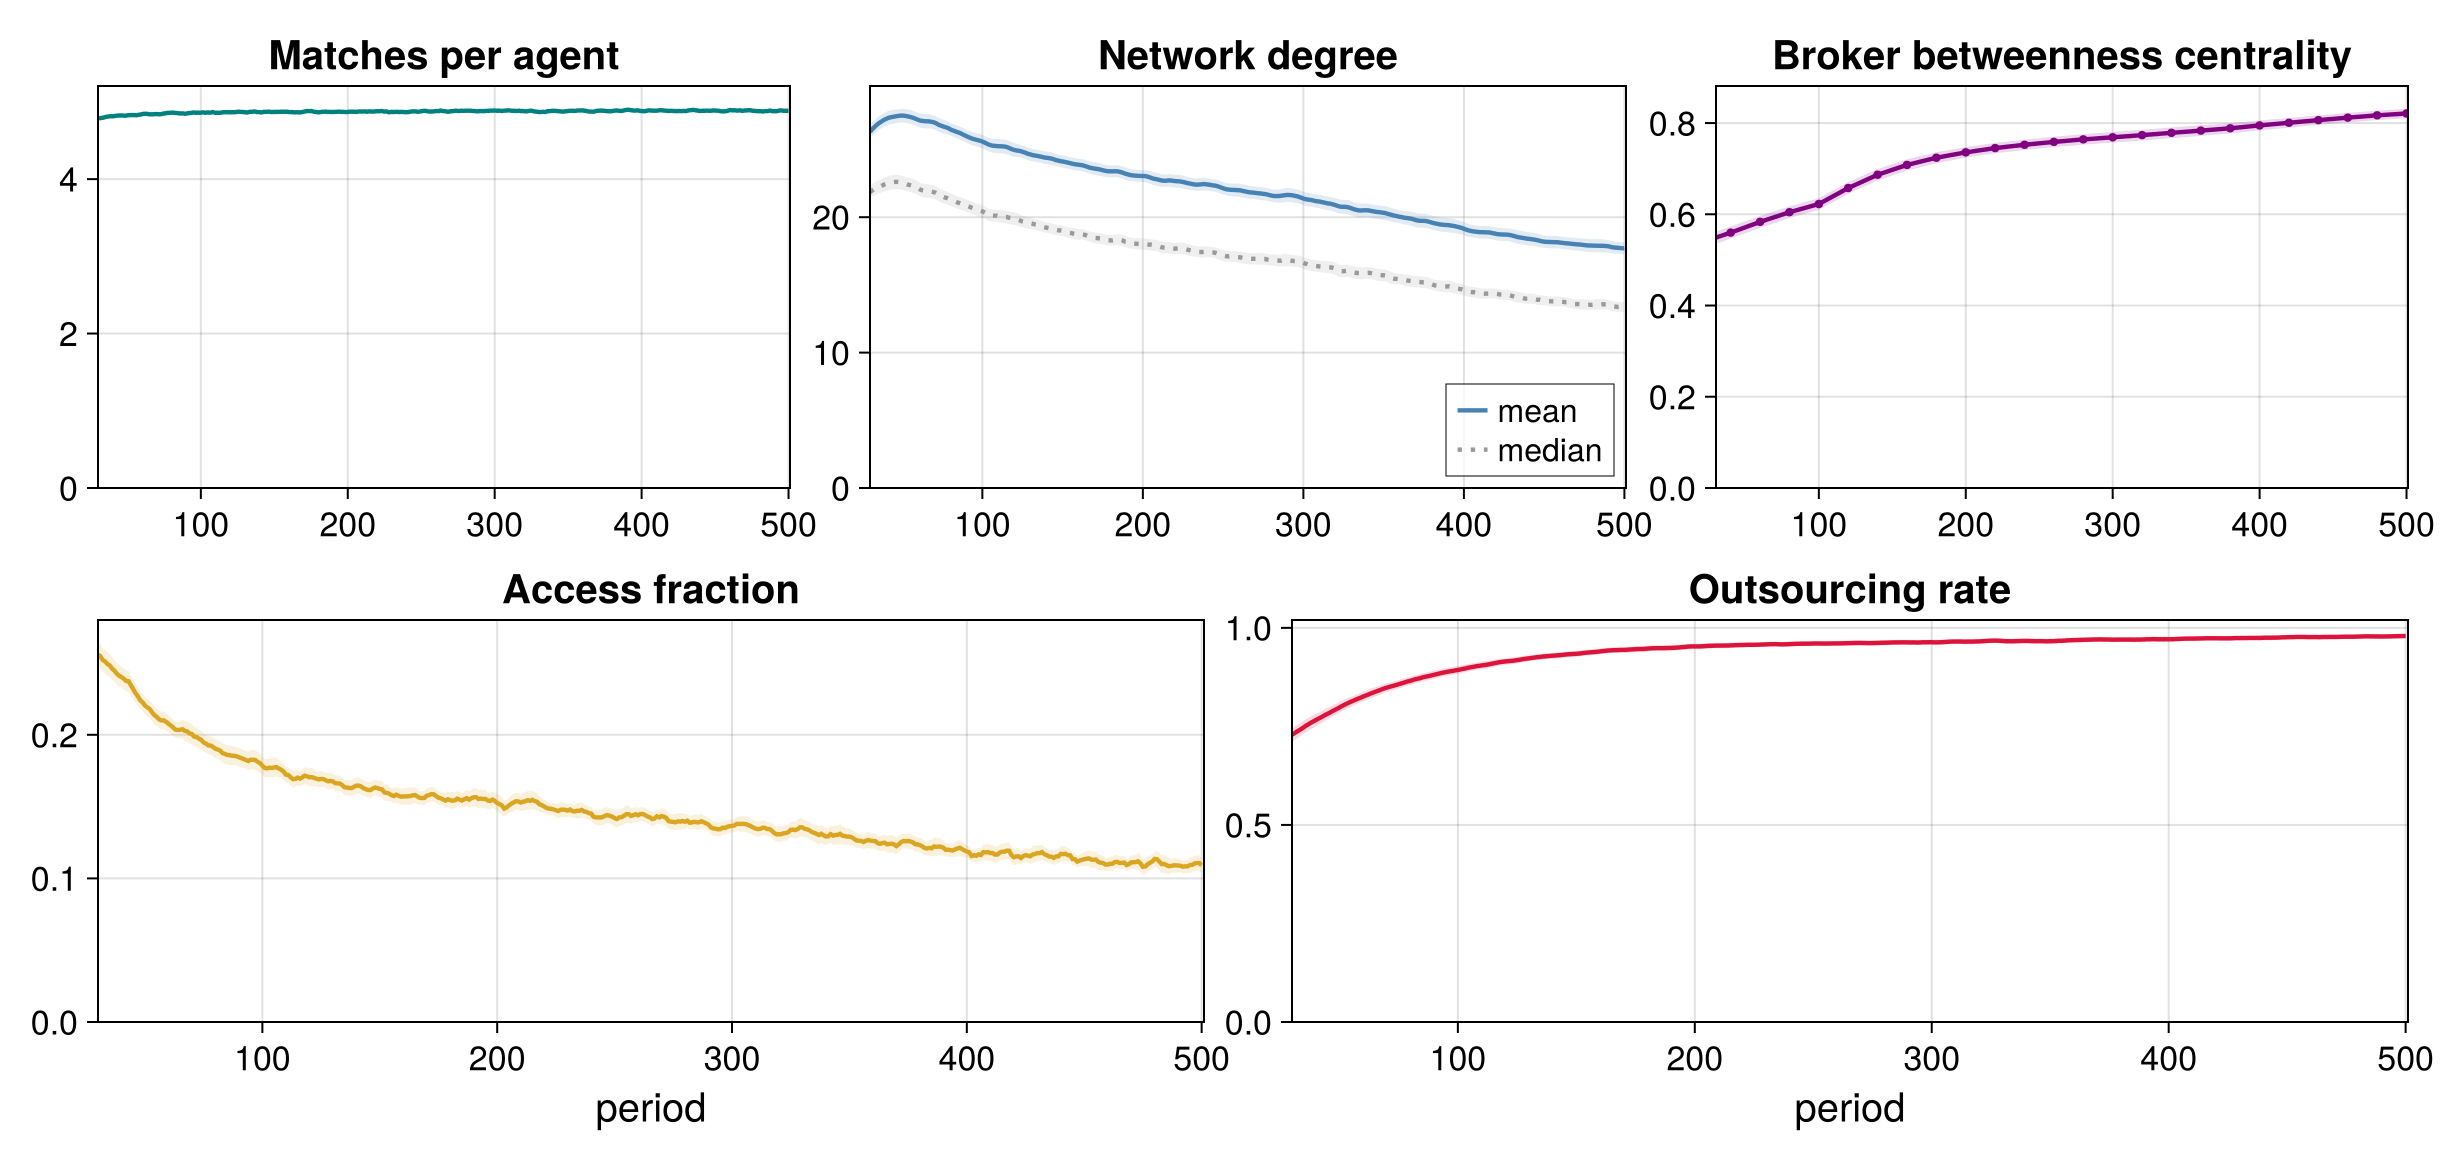
\includegraphics[width=0.75\linewidth]{figs/fig1_dynamics.png}
\caption{\textbf{Baseline dynamics.} Lines are 5-observation rolling ensemble means over seeds at the
baseline regime; shaded ribbons are pointwise 95\% Monte Carlo intervals. Some
intervals are narrower than the plotted lines and therefore are not separately
visible. Broker betweenness centrality is measured every 20
periods; the other outcomes are measured every period. Axes start at
$t=30$ to omit the initialization transient.}
\label{fig:dynamics}
\end{figure}

\begin{table}[t]
\centering\small
\caption{\textbf{Broker use, access, and assessment quality.} Early and late are ensemble
means over seeds averaged over $t\in[50,70]$ and $t\in[481,500]$; the
across-regime column reports the median late mean across the 98
regimes. Outsourcing rate is outsourced requested positions divided by all
requested positions.}
\label{tab:baseline-measures}
\begin{tabular}{lccc}
\toprule
 & \multicolumn{2}{c}{Baseline} & Across regimes \\
\cmidrule(lr){2-3}
Measure & early & late & late, median \\
\midrule
\multicolumn{4}{l}{\emph{Market use and access}} \\
\quad Outsourcing rate & $0.83$ & $0.98$ & $0.96$ \\
\quad Output gap (broker $-$ self) & $+0.02$ & $+0.65$ & $+0.52$ \\
\quad Access fraction & $0.21$ & $0.11$ & $0.11$ \\
\addlinespace
\multicolumn{4}{l}{\emph{Assessment quality}} \\
\quad Broker holdout rank correlation & $0.84$ & $0.90$ & $0.90$ \\
\quad Broker holdout $R^2$ & $0.23$ & $0.63$ & $0.40$ \\
\quad Principal holdout rank correlation & $0.55$ & $0.50$ & $0.51$ \\
\quad Principal holdout $R^2$ & $-1.99$ & $-3.16$ & $-3.32$ \\
\bottomrule
\end{tabular}
\end{table}

Widespread broker use is generally, but not always, accompanied by higher realized
output. Mean realized output is higher through the broker channel than through
self-search in 84 regimes, and the output gap (broker minus
self-search) averages $+0.49$ across regimes (late means). Paired 95\%
Monte Carlo intervals are above zero in
82 regimes and below zero in 14. The negative
gaps occur in 14 regimes, all with no or nearly no turnover
($\eta\in\{0,0.001\}$). Broker use and output differ because principals choose a
channel using satisfaction scores that include unfilled requests, fees, and search
costs, whereas the output gap compares realized output among formed matches. The
gap also reflects the candidates considered, offers made, and offers mutually
accepted. Outsourcing is therefore not itself evidence that the broker always
produces better matches.

The broker's assessment advantage appears more consistently in ranking candidates
than in predicting output levels. On a held-out sample of random partners
(Appendix~A~\S8), its rank correlation is 0.90 at the
baseline and has a median of 0.90 across regimes, compared with
0.50 and 0.51 for principals. The
broker-minus-principal difference in holdout rank correlation is positive in 96 of
98 regimes. Paired 95\% intervals are above zero in
92 regimes and below zero in only 1. The two
nonpositive point estimates occur on the hardest pure-complementarity problems
discussed below.
The broker's level accuracy is less consistent, but not uniformly poor: its
holdout $R^2$ is 0.63 at baseline, has a median of
0.40 across regimes, and is positive in
60 of 98 regimes. Candidate selection requires a
useful ordering, not an accurate prediction of each candidate's absolute output.

Within the model, the broker's core service is choosing among accessible
counterparties, not finding otherwise unreachable ones. Its ranking advantage
appears under pure general quality as well as complementarity: at $\rho=1$, the
broker-minus-principal difference in holdout rank correlation averages 0.46 and is positive in
all 11 pure-quality regimes.
The one-at-a-time checks also show that initial network degree ($k_G$), broker
roster fraction, and the number of strangers available in self-search have
comparatively small effects on the main economic outcomes.

\subsection{The Broker's Information Advantage Comes from Pooled, Pair-Level Data}

The ordering advantage does not depend on neural-network learning. When Ridge
regression replaces both neural networks, the broker-minus-principal difference in
holdout rank correlation is
0.335 at the baseline, has a median of 0.342 across
the 98 regimes, and is positive in all 98.
Supplementary Figure S4 reports the pattern across regimes and the
$\rho\times\delta$ design.
The paired-Ridge broker still has more observations and retains more information
about each pair than a principal. Three additional Ridge experiments impose the
restrictions described above. Because each restriction changes later matching and
learning, their effects need not add up.

Pooled sample size accounts for much of the advantage
(Fig.~\ref{fig:information-sources}). Across the 26 regimes
in the baseline and $\rho\times\delta$ design, the median broker-minus-principal
difference in holdout rank correlation is
0.458 under paired Ridge but only
0.065 with a size-matched broker. The size-matched difference remains
positive in 20 of 26 regimes, so
pooling is important without being the broker's only advantage.

The information retained in each observation also matters. When the broker retains
the type of only one party, the median broker-minus-principal difference in
holdout rank correlation is
-0.344 and is positive in only
6 regimes. When it retains both parties only through
the sum of their types, omitting their interaction, the corresponding figures are
-0.329 and 7. The cost of
omitting the interaction is greatest when complementarity matters; under pure
general quality, it is unnecessary. The broker's information advantage therefore
comes from both the number of observations it pools and whether each observation
retains information about both parties and their interaction, not from
neural-network flexibility alone.

\begin{figure}[t]
\centering
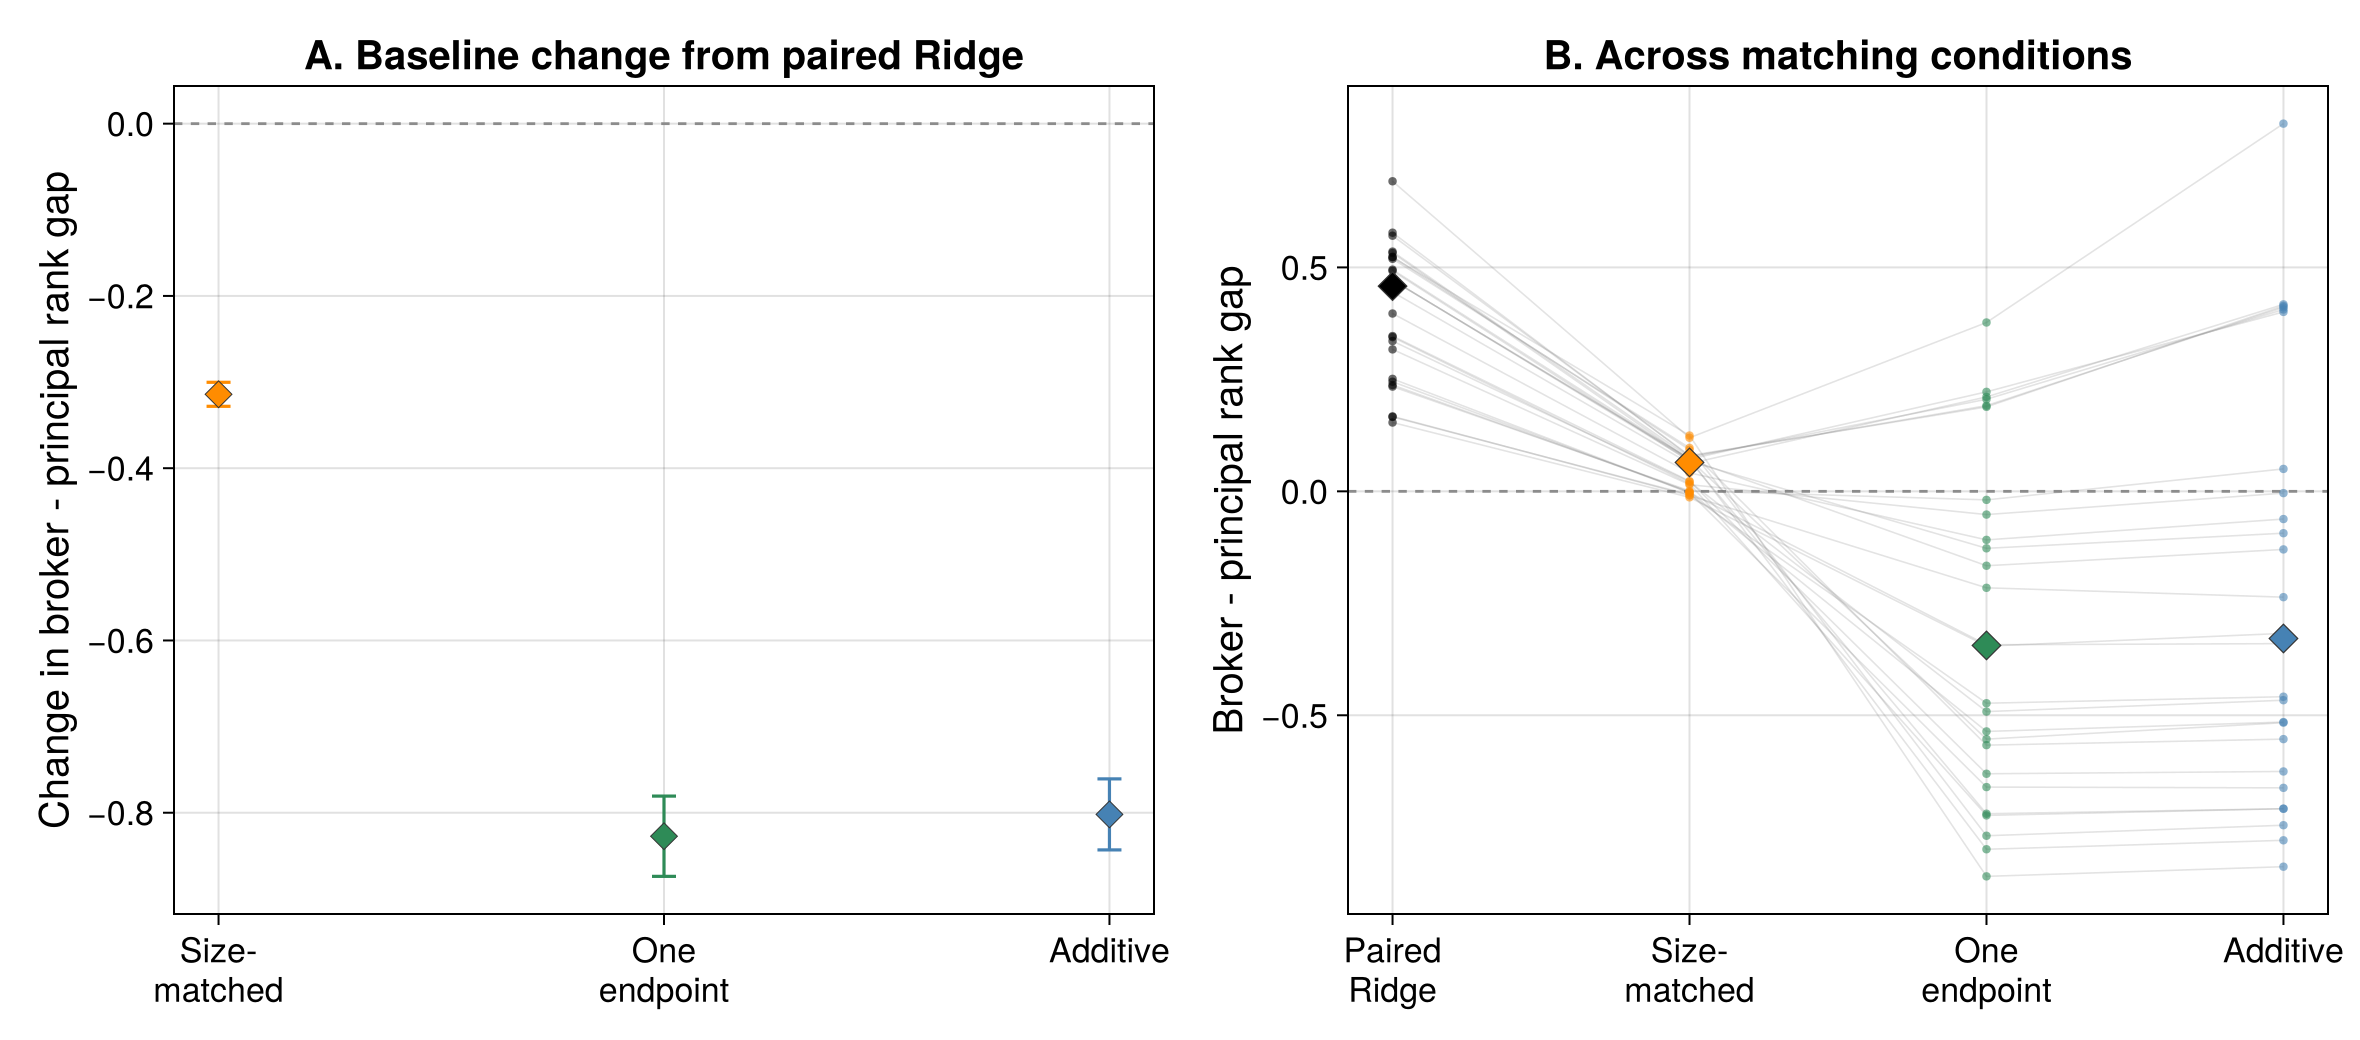
\includegraphics[width=0.94\linewidth]{figs/fig_information_sources.png}
\caption{\textbf{Sources of the broker's ranking advantage.} Panel A shows each Ridge restriction's change in the broker-minus-principal
difference in holdout rank correlation at the baseline, calculated as the
restriction minus paired Ridge. Points are mean common-seed differences; whiskers
are paired 95\% Monte Carlo intervals over 50 seeds. Panel B shows the
broker-minus-principal difference in holdout rank correlation under paired Ridge
and each restriction across the 26 regimes in the
$\rho\times\delta$ design, including the baseline. Thin lines connect estimates
for the same regime across Ridge variants, small points are regime means, diamonds
are medians, and the horizontal line marks zero.}
\label{fig:information-sources}
\end{figure}

\subsection{The Nature of the Matching Problem Shapes the Broker's Advantage}
\label{sec:matching-shapes}

Different markets present brokers with matching problems of different kinds. In
this model, $\rho=0$ gives pure complementarity and $\rho=1$ gives pure general
quality. The parameter $\delta$ increases learning difficulty by making
complementarity payoffs change more sharply across a boundary in type-pair space.
At $\rho=1$, complementarity disappears and $\delta$ has no effect. This endpoint
is therefore a separate boundary condition, not a smooth continuation of the
interior $\rho$ values. Broker centrality is governed primarily by the composition
of match value ($\rho$). Betweenness centrality falls
from 0.85 at $\rho=0$ to 0.13 at $\rho=1$, while the access
fraction rises from 0.10 to 0.17 (late means along the
one-at-a-time sweep, $\delta=0.5$). The $\rho\times\eta$ grid shows the same
relationship at every turnover rate: moving from $\rho=0$ to $\rho=0.85$ raises
access and lowers centrality. When complementarity dominates, the broker is more
central even though more of its matches re-pair principals who are already tied.

Difficulty changes the broker's informational advantage only when complementarity
contributes substantially to match value. Under pure complementarity, increasing
$\delta$ from 0 to 1 lowers the broker's rank correlation from
0.94 to 0.41 and changes the
broker-minus-principal difference in holdout rank correlation from
0.28 to -0.04
(Fig.~\ref{fig:grid}). This effect fades as $\rho$ approaches general quality and
disappears at $\rho=1$ by construction. Paired 95\% intervals for this difference are
above zero in 24 of the 26 regimes. Only
the two hardest pure-complementarity conditions depart from the
general pattern: one interval includes zero and the other is below zero. This is a
qualification to the neural-network result, not a general failure of broker
learning. With paired Ridge, this difference remains positive in every regime.

The broker's realized output advantage is greatest when match value depends on
complementarity. Paired 95\% intervals for the broker-minus-self-search output gap
are above zero in all 26 regimes, including the two hardest
pure-complementarity conditions. This does not imply that poorer holdout rankings
produce better matches. Holdout rank correlation evaluates random partner sets;
realized channel output also reflects endogenous candidate pools, offers, and
mutual acceptance. The broker's realized-output advantage survives where its
relative NN ranking advantage does not, but the results do not identify which
stage of the matching process accounts for that difference.

\begin{figure}[t]
\centering

\includegraphics[width=\linewidth]{figs/fig2_grid_lines.png}
\caption{\textbf{Outcomes across the matching problem ($\rho\times\delta$).} Six outcomes across the $\rho\times\delta$ grid; one line per difficulty level
$\delta$, each spanning $\rho=0$ through $0.85$. The pure-quality boundary
$\rho=1$, where $\delta$ has no effect, is one separate regime shown once and
unconnected. The figure therefore displays all 26 regimes in the design. Each
marker is a late-window mean over that regime's seeds; whiskers are 95\% Monte
Carlo intervals.
The reported difference in holdout rank correlation is broker minus principal;
the output gap is broker
channel minus self-search.}
\label{fig:grid}
\end{figure}

\subsection{A Broker Can Be Highly Central While Doing Little Bridging}

In most regimes, the broker's structural position strengthens over time while the
principal network thins. At the baseline, mean principal degree falls from
27.2 to 17.8, while broker betweenness centrality
rises from 0.61 to 0.83 (early to late means).
This co-movement occurs in 79 of 98 regimes,
and principal degree falls in 80 of them
(Fig.~\ref{fig:position}). In most regimes, direct ties do not accumulate fast
enough to offset turnover. The broker's structural advantage therefore does not
self-liquidate.

Assessment and access explain the composition pattern above. An access match
creates a direct tie between previously unconnected principals and can remove the
broker from their shortest path. An assessment match reuses an existing tie, so the
broker can serve the market without directly densifying the principal network.
As matching shifts toward general quality, brokered access becomes more common,
the principal network becomes denser, and broker betweenness falls sharply even
though outsourcing remains high. The broker's access work therefore creates
alternative paths even while principals continue to rely heavily on its services.
Figure~\ref{fig:position} separates this composition pattern from turnover.
Holding $\rho$ fixed, increasing turnover raises access and centrality at every
tested $\rho$. The access fraction therefore has no uniform association with
centrality. Turnover creates network gaps; matching composition determines how
often brokerage closes them with direct ties.

The turnover effect is substantial but nonlinear. Holding other parameters at
baseline, increasing $\eta$ from 0 to 0.03 lowers late mean principal degree from
85.6 to 16.6 and raises broker centrality from
0.11 to 0.84, with most of the change occurring between
$\eta=0.001$ and $0.01$. Turnover also changes realized broker value. In the
$\rho\times\eta$ grid, the 95\% interval for the broker-minus-self-search output
gap is below zero in 4 of 4 $\rho$ conditions at
$\eta=0$, but above zero in 4 of 4 by
$\eta=0.01$. In the model, turnover supplies both structural opportunities and the
conditions under which brokered matches outperform self-search.

\begin{figure}[t]
\centering

\includegraphics[width=\linewidth]{figs/fig3_position_work.png}
\caption{\textbf{Broker centrality and access fraction.} Left: broker betweenness centrality and access fraction over time at the
baseline, as 5-observation rolling ensemble means over
seeds, with pointwise 95\% Monte Carlo intervals; centrality is measured every
20 periods. Right: all 20 combinations in the $\rho\times\eta$
grid, with other parameters held at baseline, including $\delta=0.5$, each shown
as a late-window mean over that regime's seeds. Color identifies turnover $\eta$,
marker shape identifies $\rho$, and whiskers are 95\% Monte Carlo intervals on
both axes.
Within each $\eta$, lines connect $\rho=0,0.5,0.85$. The pure-quality boundary
$\rho=1$, where complementarity is absent, is shown unconnected. Time-series
panels begin at $t=30$ to omit the
initialization transient.}
\label{fig:position}
\end{figure}

The pure-quality boundary confirms that low access alone is not sufficient for high
centrality. Although higher turnover raises centrality there, centrality remains
below pure complementarity at the same turnover rate. In the tested regimes, high
centrality occurs when turnover renews network gaps and brokerage mainly assesses
existing relationships. Because access remains low overall and declines within
runs, brokerage does little to eliminate the structural basis of its own position.

\begin{figure}[t]
\centering
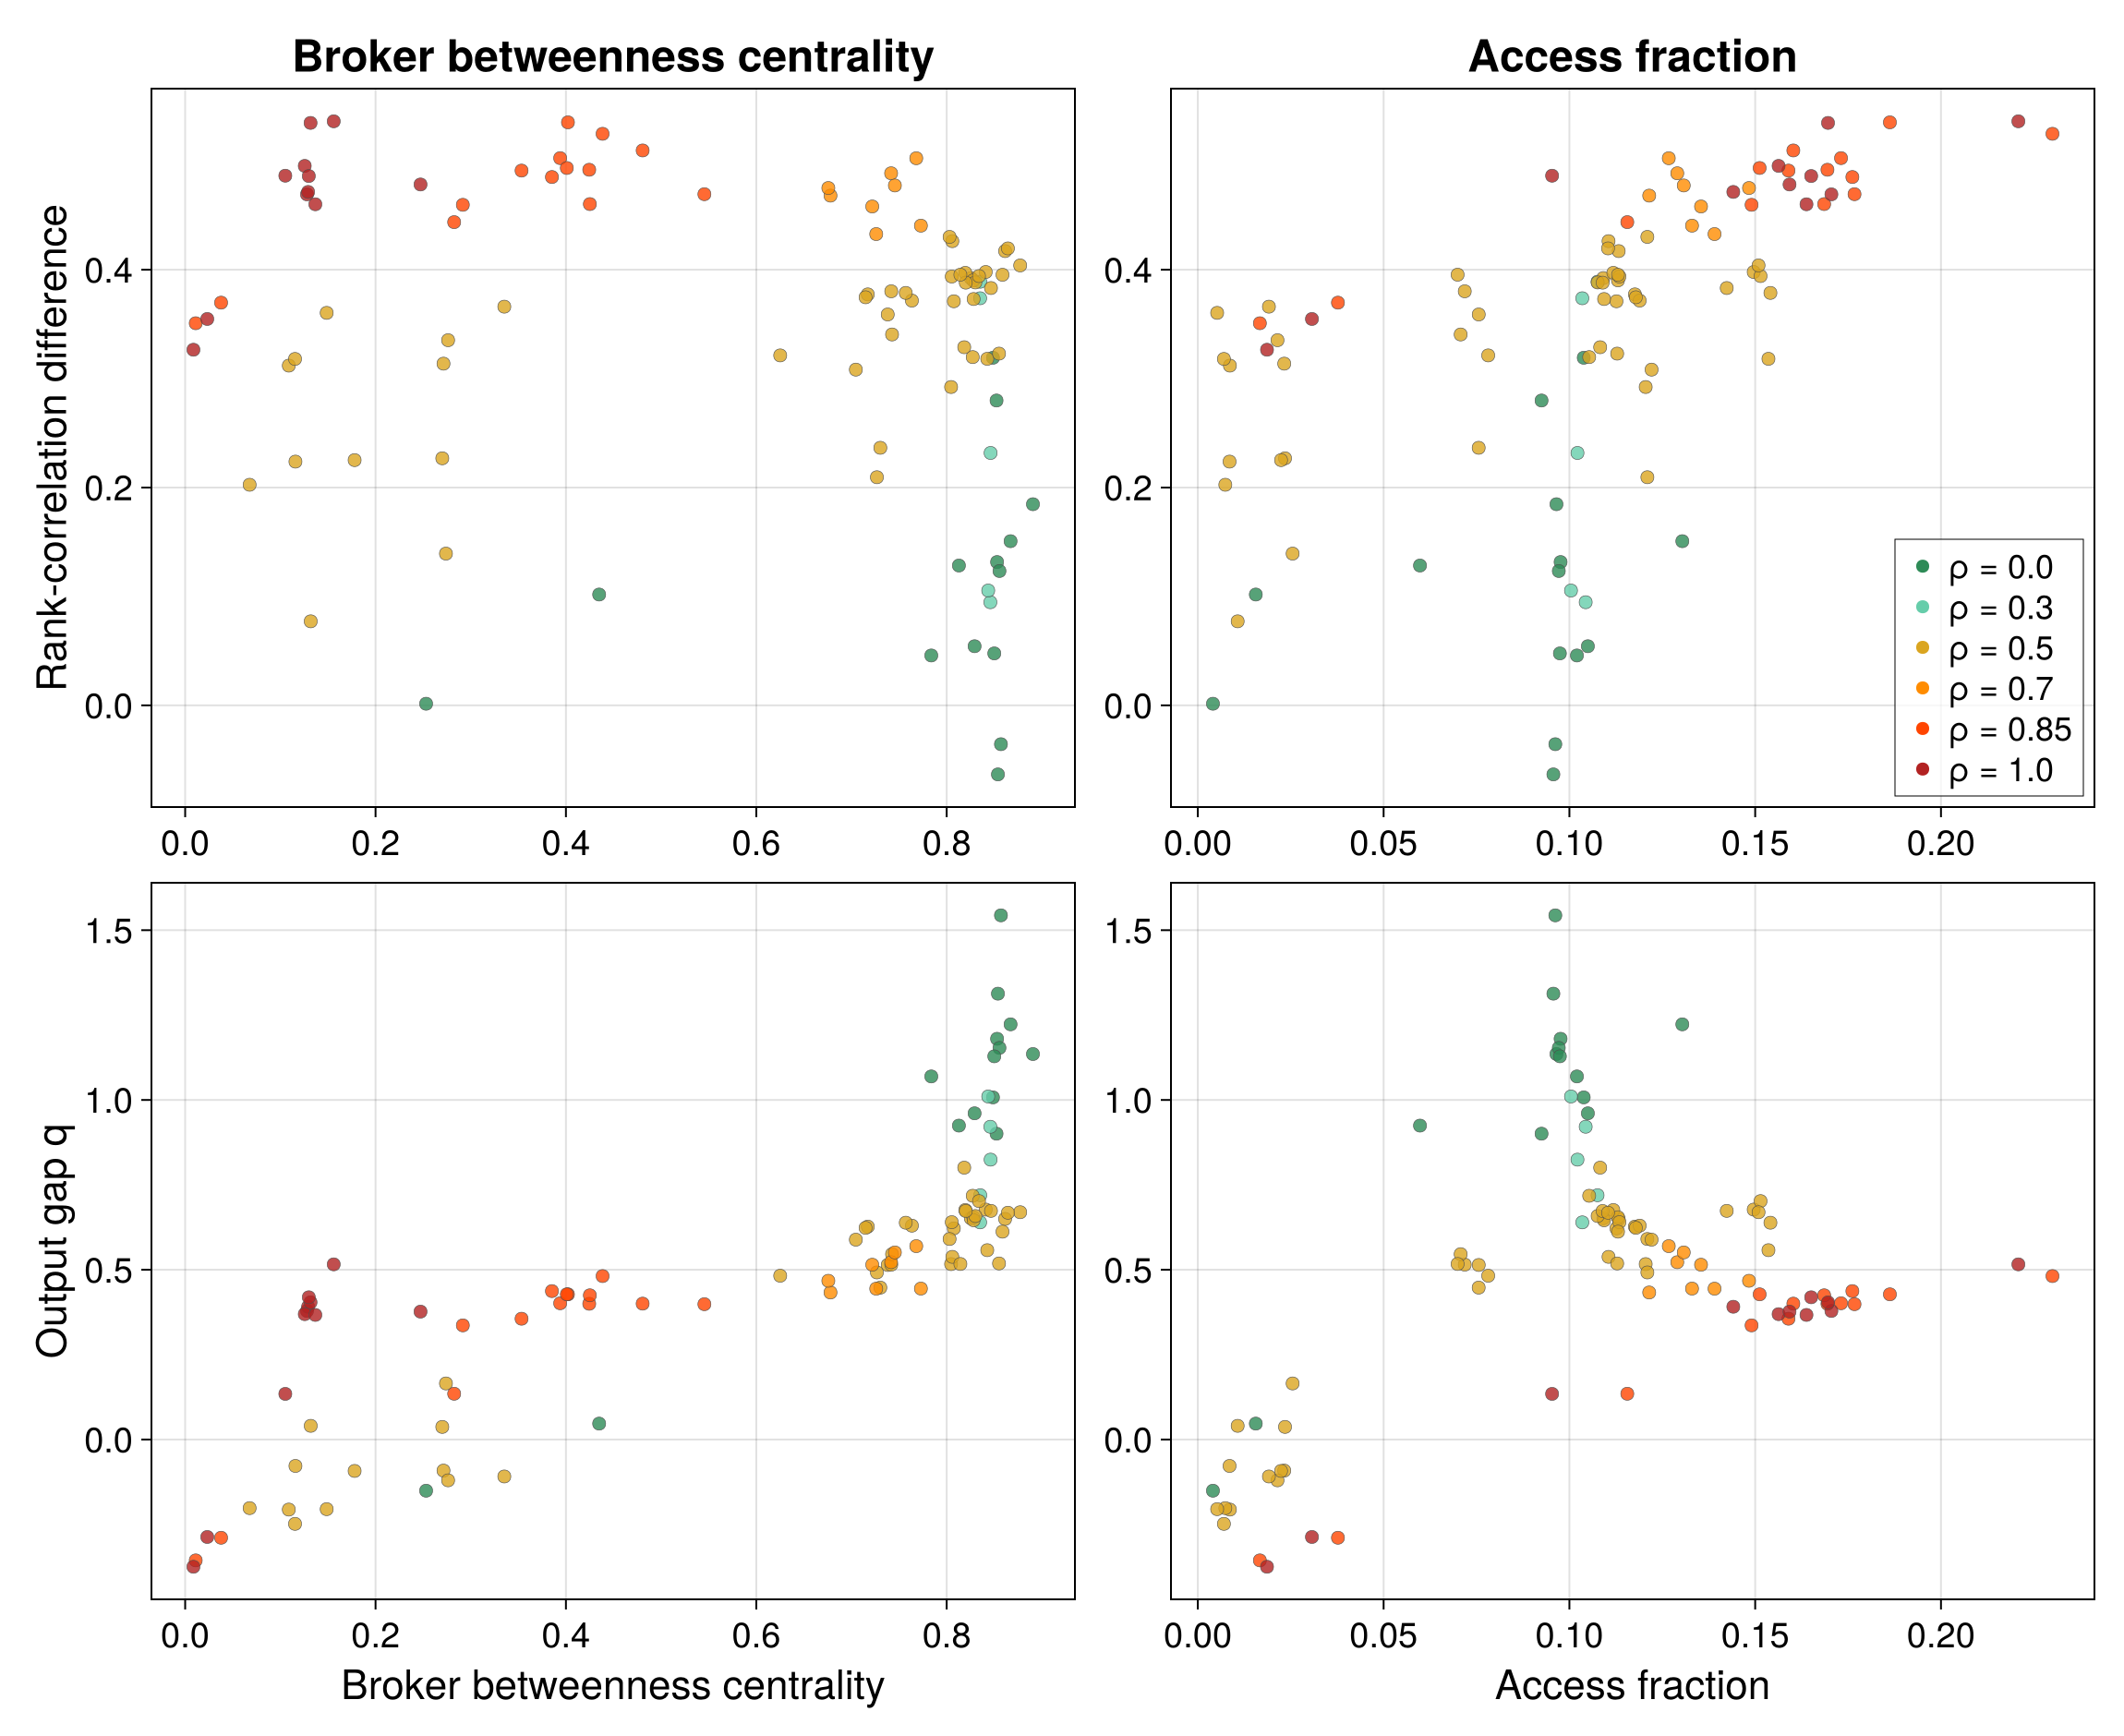
\includegraphics[width=0.92\linewidth]{figs/fig4_advantage.png}
\caption{\textbf{Ranking and output differences by centrality and access.} Difference in holdout rank correlation (broker minus principal) and output gap
(broker channel minus self-search) against broker betweenness centrality and
access fraction; one dot for each of the 98 effective regimes, each a
late-window mean over its seeds. Color identifies matching composition $\rho$.}
\label{fig:advantage}
\end{figure}

Figure~\ref{fig:advantage} shows that structural position relates differently to
relative ranking and realized value. Across otherwise matched parameter settings,
moving from pure complementarity to pure general quality reduces the output gap from
+0.87 to +0.23, while increasing the
broker-minus-principal difference in holdout rank correlation from
0.10 to
0.46. The broker is therefore most central and produces its
largest realized-output advantage where its relative holdout-ranking advantage is
smaller. Taken together, the results separate the sources of informational,
economic, and structural advantage: pooled pair-level data improves ranking,
complementarity raises broker value, and turnover renews the network gaps that
sustain centrality. These advantages need not move together.

\subsection{Propositions}

The simulation results motivate the following falsifiable propositions for
future empirical research. These propositions extend the model's implications
beyond the simulated setting:

\noindent\textbf{P1.} In complex matching markets, brokers add value primarily by
assessing complementarity among reachable counterparties, not by bridging
disconnected parties.

\noindent\textbf{P2.} A broker's betweenness centrality is produced by outsourcing
volume and client satisfaction, it tracks how much complementarity matters to match
value, and assessment-heavy brokers tend to retain or gain centrality as networks
evolve.

\noindent\textbf{P3.} Bridging position and bridging behavior are generally
negatively related across markets: the most central brokers tend to do less
bridging, except where turnover continually creates new network gaps for them to
bridge.

\noindent\textbf{P4.} Broker predictive advantage tracks the complexity of learning
the complementarities relevant to match value, and it can diverge from structural
centrality.


\section{Transient Brokerage and Its Conditions of Possibility}
\label{sec:transient-brokerage}

Outsourced relational work performed at scale by corporate brokers creates the conditions under which the broker can transition from intermediary to principal. The broker dismantles the relational package previously negotiated with its clients and replaces it with a new configuration organized around the broker's ownership of the resources it used to intermediate (\emph{resource capture}), or the monetization of the information generated through prior matching activity (\emph{data enclosure}).

These configurations are two qualitatively different forms of capture, which can be pursued in parallel and along with standard brokering. In \emph{resource capture}, the broker takes inventory risk and starts acting as a principal in the market it used to intermediate. Counterparties interact with the broker only, without creating direct ties between each other. As the broker expands its principal activity and shrinks its matching services, former clients become counterparties or competitors. In \emph{data enclosure}, the broker monetizes information directly by selling predictions, analytics, or other information services, often as a subscription.

What makes capture possible, I suggest, is primarily the broker's information advantage, not its structural position. Structural and informational advantages are decoupled, and capture may occur even if the broker's centrality is declining. This is because constructing viable relational packages generates an informational byproduct that the broker can leverage. Two features of the broker's informational landscape, established through repeated matchmaking at scale, facilitate capture: cumulative knowledge of complementarities coming from the \emph{outsourced} nature of its relational work, and information infrastructures arising from its \emph{corporate} nature; both of which, other actors cannot easily replicate.

\emph{(i) The role of complementarity information.} The broker's vicarious work generates knowledge of how different parties pair together, what kinds of matches succeed across the market, and what relational packages support different transactions. For regular market actors, this complementarity information is hard to replicate. Unlike attributional information about the general quality of counterparties, which any actor with sufficient market exposure can in principle acquire, complementarity information is generated through the repeated observation of various pairings. The broker holds it because it does the matching for a variety of clients; clients, who experience only their own matches, do not---unless they purchase or otherwise acquire it. Complementarity information supports resource capture, because it allows the broker to identify which resources or counterparties are most likely to generate profitable matches, so that it can capture them strategically and offload them gainfully. Complementarity information also supports data capture because it can be packaged into prediction or analytics products and services.

\emph{(ii) The role of information infrastructures.} The corporate broker's information infrastructure explains \emph{how} its information advantage can be preserved and converted. The taxonomies, classification systems, contractual templates, and algorithmic sorting procedures that the broker develops to perform vicarious work at scale and in a distributed manner, through the everyday work of its employees and representatives, are also the infrastructures through which capture can be realized. They can be repurposed to route resources to the broker itself, to put these resources back in circulation profitably, or to organize data into a marketable product. Moreover, the corporate form gives the broker the legal privileges required to build, own, and protect these infrastructures over time \autocite{colemanAsymmetricSociety1982,pistorCodeCapitalHow2019}.

These features, and transient brokerage itself, can be found in a wide variety of real-life markets. To make things more concrete, I provide two examples below, one for each configuration.

\emph{Dealers in collectible markets}. Collectors of art, fine wine, rare books, or similar specialty goods may seek trades through broker dealers who know the market. Each collector has distinct tastes and holdings; match quality depends on multidimensional complementarity between what one party has and what another wants. Dealers accumulate knowledge of collector preferences across transactions, and they may decide to leverage it and start holding inventory, for instance, by launching and operating a gallery.

\emph{Interdealer brokerage in over-the-counter (OTC) financial markets}. Interdealer brokers (IDBs) are specialized intermediaries in OTC financial markets (e.g. bond markets, foreign exchange, commodities). IDBs help institutions like banks and dealers conclude large, complicated, or anonymous transactions in the absence of a centralized trading place. They solve a hard matching problem: the right counterparty for a trade depends on inventory positions and risk appetites that parties wish to keep secret. IDBs must know who wants what at any given moment, they negotiate price across hidden order interest, they preserve anonymity until execution, and they manage long-term relationships with clients to remain included in the order flow. The complementarity information they accumulate, about who will absorb what positions at what price under what conditions, is substantial. Resource capture, however, faces regulatory and reputational hurdles. Instead, IDBs have monetized accumulated information through data divisions that package historical OTC pricing and other data products, and sell them to the same dealers whose trades generated the data and to a wider set of buy-side firms and regulators \autocites[see e.g.][]{CapitalMarketsIndicative,ARA_FullReport}.

In summary, three elements enable capture or enclosure: a matching problem that makes complementarity information valuable, an informational advantage accumulated through repeated vicarious relational work, and an institutional architecture that allows that information to be aggregated, organized, and protected.

\section{Discussion}

\subsection{Structural Advantage as a Product of Relational Work}

Within the agent-based model, the broker's centrality is a product of its relational work. The broker is central because many principals outsource to it repeatedly, which they do because its assessments are good. Its centrality rises and falls with outsourcing and satisfaction, not with exogenous features of the initial graph.

With the production of structure, two patterns emerge that pre-existing theory may not have predicted. The first is that the broker tends to be most central exactly where it bridges least in practice. Across the regimes examined, centrality is negatively associated with the access fraction (Figure~\ref{fig:position}): in the complementarity-dominated markets where the broker is most prominent, almost all its matches re-pair principals already tied to one another. A strong bridging position coincides with weak bridging behavior. Occupying a strategic position and using it for one's work are different things that theory should not conflate.

The second pattern is about the sustainability of brokerage. A long-standing expectation in the tradition is that brokerage tends to be self-undermining \autocite{burtStructuralHolesSocial1992,burtBridgeDecay2002a,stovelStabilizingBrokerage2011}. Each successful introduction densifies the network and dissolves the structural hole that gave the broker its advantage. Where the work is assessment, however, it leaves the network no denser than it found it. Across the simulations, access work is low and declining over time, so the broker\textquotesingle s structural advantage tends to persist. Self-liquidation is a feature of access brokerage. Meanwhile, the assessment-heavy brokerage characteristic of complementarity-based matching markets is more durable.

The results also suggest a precise mechanism for the decoupling of structural and informational advantage posited in Section~\ref{sec:transient-brokerage}. The two answer to different features of the matching problem. The broker's structural prominence tracks the composition of match value, rising as matching becomes more complementarity-driven, while its prediction edge tracks the complexity of the complementarity component, which can vary independently. A broker can be highly central despite a modest informational lead or hold a decisive informational lead from an unremarkable position. Betweenness centrality is best understood not as a static measure of opportunity but as a product of the relational work the broker performs.

\subsection{Scope Conditions and Generalizability}

The concept of transient brokerage applies most directly to matching markets in which (i) matching is complex enough that the value of a match depends not only on the general quality of each party but also on their complementarity and (ii) a corporate broker operates as a repeat-player accumulating information across transactions. The further a case departs from these conditions, the weaker the predictions of the theory. When the relational dimension is weak, the broker's advantage rests primarily on data volume about multiple counterparties, making its informational position less privileged. When the broker is a physical person, she lacks the temporal persistence, infrastructural capacity, and legal architecture that the corporate broker relies on.

The dynamics of transient brokerage also depend on the nature of the brokered resource and the institutional environment. In a goods market where items are bulky and physical delivery is required, the costs and logistics of capture look very different, compared to a market for services, or a market where goods are virtual or ownership passes without physical possession. In some markets, regulation may slow or prevent capture. Market structure matters as well. The model considered in this article features a single broker. With multiple brokers competing for the same clients or matches, the cross-market data pool is fragmented, and each broker may accumulate a smaller informational advantage, unless one or a few dominate the others. A systematic treatment of broker competition is deferred to future work.

Transient brokerage is relevant to a particular configuration of brokerage, in which matching problem, corporate form, and information accumulation give rise to a distinctive trajectory. The sociological literature has used brokerage to describe a wide range of phenomena, from immigrant children translating for their parents to marriage matchmakers and political brokers. The relational-work view of brokerage developed in this article can be applied to what many of these so-called brokers do. Without the repeat-player structure of corporate brokerage, the legal and infrastructural architecture of the firm, and an economic matching problem complex enough to sustain an informational advantage, however, the pathway to capture is not the same.

These scope conditions point to candidate domains in which to validate the theoretical propositions. Real estate and various types of financial intermediation, including interdealer brokerage, combine complex matching, corporate repeat-player brokers, and meaningful complementarity information. Import-export management and data markets also share many of these features.

\subsection{The Political Economy of Corporate Intermediation}

The corporate broker is a vehicle for the accumulation of information generated by the interactions between others, and the principals whose matching activity produced the information do not participate in the profits. The asymmetries that make capture possible are not just a byproduct of a broker's size or expertise. They are legally constituted. Corporate brokers assemble cross-market data and build classification systems and information infrastructures under the legal protections of the corporate form, which allows vicarious relational work to solidify into a durable informational moat. Whether a broker can convert its informational position into resource ownership or data provision depends on the institutional environment as much as on network position.

The simulations make the distributional stakes of transient brokerage concrete. When the broker becomes a principal, it changes who gets connected to whom. The principals observe many fewer matches than they otherwise would, and most matches in the market teach them nothing at all. The informational asymmetry that makes capture possible is widened by capture itself: the broker takes control not only of the resource but of the data its placement generates. Transient brokerage shifts how value is distributed, channeling the returns of participants' collective relational activity to the corporations who record and mine the data it generates.

Capture by corporate brokers has become more common since the 1980s alongside three transformations that have reshaped market intermediation: the turn to finance, which expanded the share of economic activity routed through specialized intermediaries \autocite{carruthersFinancializationInstitutionalFoundations2015,krippnerCapitalizingCrisisPolitical2011}; the digital turn, which dramatically lowered the cost of accumulating, storing, and analyzing the data that brokerage generates while also expanding the demand for predictive analytics \autocite{cohenTruthPowerLegal2019,gandyPanopticSortPolitical1993}; and the rise of platform capitalism, which produced multi-sided market operators that own the relational infrastructure of matching while monetizing the data it generates \autocite{sadowskiInternetLandlordsDigital2020,viljoenDesignChoicesMechanism2021}. Transient brokerage is one of the mechanisms that link these transformations together and contributes to a broader shift in how value is extracted from economic activity.

Significant evidence exists in the literature that, across financial markets, corporate brokers that once facilitated matches between others have, indeed, increasingly become principals, either by capturing the activity they used to intermediate or by monetizing data. In financial markets, the demutualization of stock exchanges is a prime example. As late as the mid-1990s, almost all major global exchanges operated as member-owned mutual organizations. By the mid-2000s, a majority had introduced electronic trading systems that allowed them to grant trading access directly to investors, bypassing the services of member firms, and had converted to for-profit shareholder structures \autocite{aggarwalDemutualizationCorporateGovernance2002,petryNationalMarketplacesGlobal2021}. For-profit exchanges now derive a growing share of revenue from proprietary data feeds and trading technology \autocite{mackenzieTradingSpeedLight2021,pardo-guerraAutomatingFinanceInfrastructures2019}.

A parallel transformation has taken place in interdealer brokerage for over-the-counter (OTC) markets, where the data divisions of prominent brokers now generate substantially higher operating margins than the broking activities themselves; this is the case, for instance, of the Parameta Solutions data division of TP ICAP, the largest interdealer broker \autocite{ARA_FullReport}. In consumer markets, Visa offers another example. Reorganized in 1970 as a member-owned cooperative of issuing banks, Visa operated for decades as a non-profit utility that brokered payment authorizations between cardholders, merchants, and banks \autocite{stearnsElectronicValueExchange2011}. Following its 2007 restructuring and 2008 IPO, Visa converted into a for-profit corporation that now derives substantial revenue from data, analytics, and risk solutions services, alongside the network and processing fees generated by its core authorization and clearing activities \autocite{VisaAnnualReport}.

\section{Conclusion}

The very conditions that make brokerage possible and valuable, such as the scarcity of information and the complexity of the matching problem, create opportunities for the broker---particularly the corporate broker---to take control of resources. At the transition point, the broker dismantles the relational package that was negotiated with its principals and lets the boundary between \emph{vicarious} and \emph{personal} relational work collapse, for its economic advantage. It abandons the service-tie configuration that existed and (re)negotiates a new relationship (with the same principals or new ones), one that is premised on the broker's direct ownership and control of formerly brokered resources or of the data streams they generated. In the latter case, the accumulated data can also be mined internally or licensed out to feed proprietary behavioral prediction, classification, and scoring products \autocite{fourcadeSeeingMarket2017,fourcadeOrdinalSociety2024} for use in markets distinct from those in which they originated \autocite{viljoenRelationalTheoryData2021,zuboffAgeSurveillanceCapitalism2019}.

This article helps explain why the digital turn has facilitated broker capture at scale. Because information is central to brokerage, changes in the information ecosystem reshape the conditions under which transient brokerage becomes available, and digital technology has changed those conditions decisively. Relational infrastructures that once consisted of internal handbooks, contractual templates, and bureaucratic procedures now incorporate data taxonomies, algorithmic sorting, and interface designs that constitute the relational packages they administer in real time and at scale. The asymmetries that make capture possible are correspondingly amplified, and the pathway from accumulated information to ownership or monetization, shorter.

\subsection{Digital Platforms and Automated Matching}

Transient brokerage is intimately related to the rise of digital platforms and algorithmic marketplaces, from gig economy apps to electronic exchanges, that partly automate the work of matching. Where brokers perform vicarious relational work on behalf of their clients, platform operators design mechanisms to automate and circumvent relational work, typically through auction protocols, ranking algorithms, and rating systems. The platform operator does not match buyer and seller; it builds the apparatus that matches them and extracts fees or data flows from the result.

In some markets, mechanism design substitutes for relational work. In others, it absorbs and reshapes relational work, with the platform operator administering the categories, ratings, and defaults that constitute the relational packages on behalf of both sides. These arrangements are not brokerage, but something different. The dynamics of their emergence share important features with transient brokerage: the platform operator accumulates cross-market information about its users, holds infrastructural and legal advantages that make this accumulation difficult to challenge, and is often well positioned to transition from automating matches to selling matched resources or analytics about them.

For example, Amazon operates as both a marketplace for third-party sellers and a direct retailer of its own products. Zhu and Liu \autocite*{zhuCompetingComplementorsEmpirical} tracked over 150,000 product listings initially supplied by third-party sellers and found that Amazon began directly selling roughly three percent of them over the following ten months. The platform was significantly more likely to enter listings with higher sales and better customer reviews, using information available to it as the marketplace operator. Khan \autocite*{khanAmazonAntitrustParadox2016,khanSeparationPlatformsCommerce2019} argues that platform operators in this position are best understood not as intermediaries but as integrated firms whose control of the matching infrastructure gives them a structural advantage over the sellers they host. The same configuration recurs beyond Amazon, across leading platform firms: their business model becomes that of a lean platform that owns and profits from the matching infrastructure while pushing the underlying productive activity and capital risk onto third parties \autocite{rahmanRisePlatformBusiness2019}.

\subsection{Future Directions}

Two main directions warrant future work. On the modeling side, the ABM developed here is exploratory. It has many interacting components and considerable researcher degrees of freedom in its specification, and it carries the usual caveats of this kind of hand-crafted simulation: its results illustrate the theory rather than establish it. Systematic investigation of the parameter space, the decision rules, and the model's sensitivity to them may surface dynamics that the results presented in this article do not reveal. The research capture and data enclosure mechanisms are introduced theoretically but not formalized; they are a natural next step for an extension. On the theoretical side, the framework does not yet fully address how platforms and algorithmic marketplaces reshape the dynamics of brokerage by automating the vicarious relational work that brokers historically performed. Both directions point toward the same underlying question about the impact of the digital turn on brokerage, the institutions that rely on it, and the actors that perform it or benefit from it.

The digital turn has brought about a series of transformations. The informational byproduct of relational matching has come to rival the value of the matches themselves. Relational work is increasingly performed for the data it generates and increasingly performed by machines rather than people. The informational asymmetry between brokers and their principals has widened. Existing relational packages are being dismantled to extract value from the information and infrastructures associated with them. These shifts redraw the boundaries on which brokerage rests: between internalized and outsourced relational work, and between vicarious and personal relational work. Brokerage becomes a transient position, held so long as brokering remains more profitable than capture.

% These four references appear in the generated ABM results section, which the
% Word source represents with an ellipsis. Retain them until that section is
% inserted so this bibliography matches the Word manuscript's 62 entries.
\nocite{borgattiStructuralHolesUnpacking1997,brandesFasterAlgorithmBetweenness2001,everettUnpackingBurtsConstraint2020,freemanSetMeasuresCentrality1977}
\printbibliography[heading=bibnumbered,title={References}]

\end{document}
